% Intro ===================================================================================
\begin{frame}
	\section{Introduction}
	\setbeamercolor{block title example}{use=structure,fg=white,bg=blue!80!black}
	\begin{beamercolorbox}[rounded=true]{block title example}
		\centering
		\LARGE
		Introduction
	\end{beamercolorbox}
\end{frame}

\begin{frame}
	\frametitle{Introduction}
	\framesubtitle{Wheeled Mobile Robot and Navigation}
	Wheeled Mobile Robot is widely used in the field. Autonomous Navigation is one of the main subject in mobile robot study.
	\begin{figure}
		\caption{Mobile Robot Application}
		\centering
		\begin{minipage}{0.3\linewidth}
			\centering
			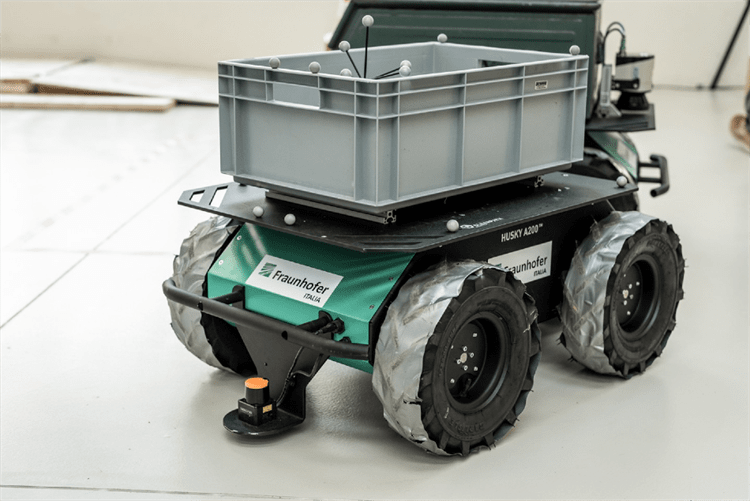
\includegraphics[scale=0.14]{image/WMR_HuskyA200.png}\footnotemark
		\end{minipage}%
		\begin{minipage}{.3\linewidth}
			\centering
			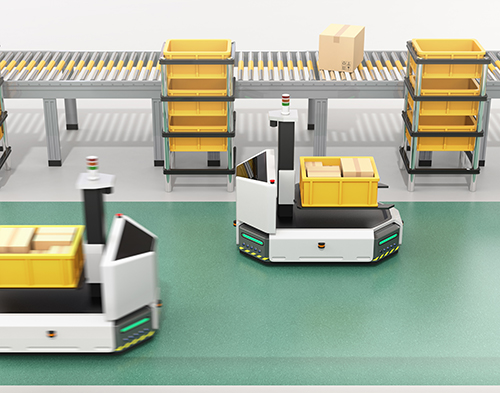
\includegraphics[scale=0.8]{image/nidec}\footnotemark
		\end{minipage}
		\begin{minipage}{.3\linewidth}
			\centering
			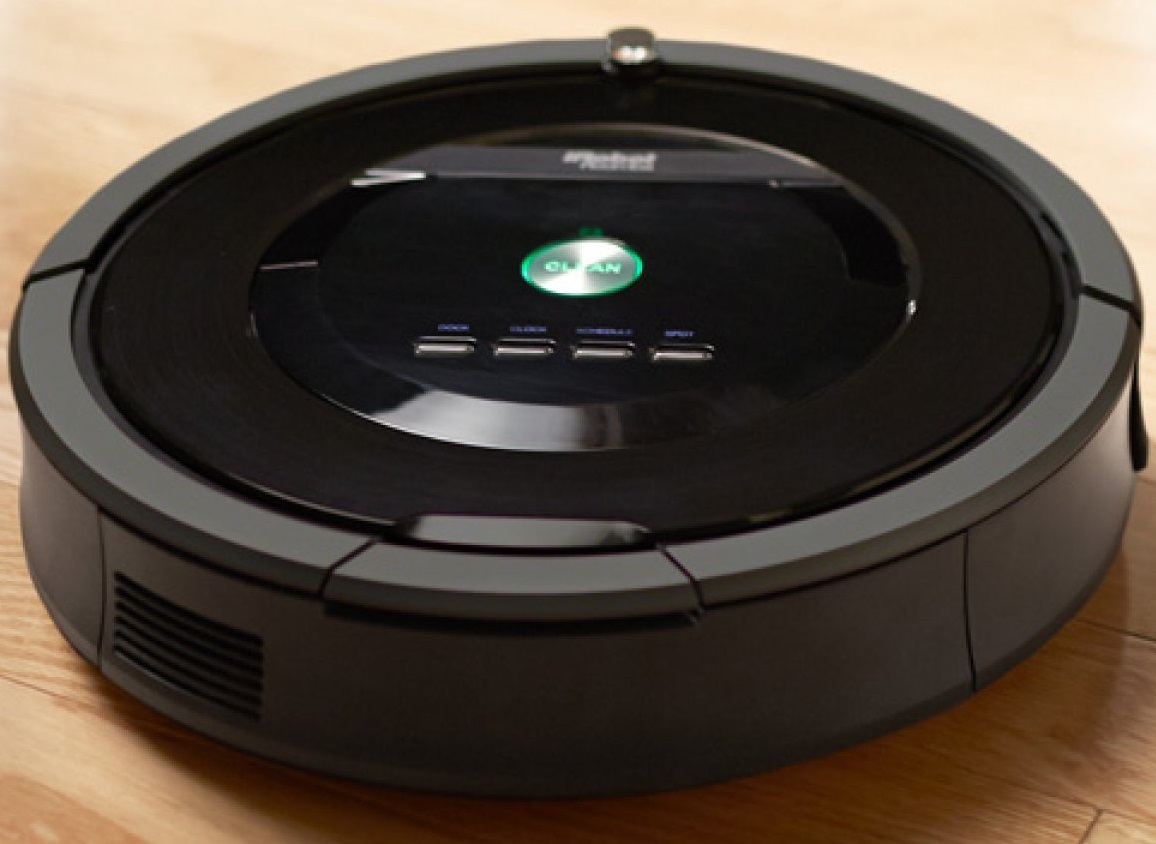
\includegraphics[scale=0.12]{image/roomba}\footnotemark
		\end{minipage}
	\end{figure}
\footnotetext[1]{HuskyA200}
\footnotetext[2]{Nidec AGV}
\footnotetext[3]{Roomba}
\end{frame}


\begin{frame}
	\frametitle{Introduction}
	\framesubtitle{Wheeled Mobile Robot and Navigation}
	To achieve an autonomous navigation functionality, it needs:
	\begin{itemize}
		\item Sensors data
		\item Algorithms
	\end{itemize}
	% talk about : All this will allow the robot to move inside surrounding with little to no human command.
\end{frame}


\begin{frame}
	\frametitle{Introduction}
	\framesubtitle{Literature Review}
	There are multiple ways of represent the surrounding environment and method of path planning.\\
	\hspace{\linewidth}\\
		\begin{columns}[T]
		\begin{column}[T]{.4\textwidth}
		Environment Representation
		\begin{itemize}
			\item Graph Representation
			\item Cell Decomposition
			\item Roadmap
			\item Potential Field
			\item -etc
		\end{itemize}
		\end{column}
		\begin{column}[T]{.6\textwidth}
		Path Planning
		\begin{itemize}
			\item Probabilistic Road Maps (PRMs)
			\item Visibility Graph
			\item Rapidly Exploring Random Tree (RRTs)
			\item Generalized Voronoi Diagram
			\item A*
			\item -etc
		\end{itemize}
	\end{column}
	\end{columns}
\end{frame}


\begin{frame}
	\frametitle{Introduction}
	\framesubtitle{Objectives}
	In this research, we aim to:
	\begin{itemize}
		\item<1-> Determine \textbf{pathway} to move the robot using \textbf{Occupancy Grid Map}
		\item<2-> Design a \textbf{controller} for the robot to follow the planned pathway
	\end{itemize}
\end{frame}



\begin{frame}
	\frametitle{Introduction}
	\framesubtitle{Scope}
	In this research:
	\begin{itemize}
		\item<1-> \textbf{Differential Drive Mobile Robot} is used
		\item<2-> \textbf{2D} environment
		\item<3-> \textbf{Simulation} is conducted using \textbf{Gazebo} and \textbf{ROS} software
		\item<4-> The project produce a \textbf{ROS} package
	\end{itemize}
\end{frame}